\documentclass[a4paper, 11pt]{article}

\usepackage[czech]{babel}
\usepackage[utf8]{inputenc}
\usepackage[left=2cm, top=3cm, text={17cm, 24cm}]{geometry}
\usepackage{times}
\usepackage{multirow}
\usepackage[ruled, czech, linesnumbered, noline, longend]{algorithm2e}
\usepackage{graphics}
\usepackage{pdflscape}

\begin{document}

% spravi problem s clinem
\catcode`\-=12

\begin{titlepage}
        \begin{center}
            \Huge
			\textsc{Vysoké učení technické v~Brně} \\
			\huge
			\textsc{Fakulta informačních technologií} \\
			\vspace{\stretch{0.382}} % zarovnani na fibo
			\LARGE
			Typografie a~publikování\,--\,3.~projekt \\
			\Huge
			Tabulky a~obrázky
			\vspace{\stretch{0.618}} % zarovnani na fibo
		\end{center}

		{\Large
			\today
			\hfill
			Petr Vitula
		}
\end{titlepage}

% sekce uvodni stranka
\section{Úvodní strana}
Název práce umístěte do zlatého řezu a nezapomeňte uvést dnešní datum a vaše jméno a přijmení.


% sekce tabulku
\section{Tabulky}
Pro sázení tabulek můžeme použít buď prostředí \verb|tabbing| nebo prostředí \verb|tabular|.


% subsekce tabbing
\subsection{Prostředí\texttt{ tabbing}}
Při použití \verb|tabbing| vypadá tabulka následovně:

% tabbing prostredi
\begin{tabbing}
        Vodní melouny \quad	\= \textbf{Cena} \quad	\= \textbf{Množství}	\kill
		\textbf{Ovoce}		\> \textbf{Cena}		\> \textbf{Množství}	\\
		Jablka				\> 25,90				\> 3 kg					\\
		Hrušky				\> 27,40				\> 2,5 kg				\\
		Vodní melouny		\> 35,--				\> 1 kus				\\
\end{tabbing}
Toto prostředí se dá také použít pro sázení algoritmů, ovšem vhodnější je použít prostředí \verb|algorithm| nebo \verb|algorithm2e| (viz sekce~\ref{section:algoritmy}).


% subsekce tabular
\subsection{Prostředí tabular}
Další možností, jak vytvořit tabulku, je použít prostředí \verb|tabular|. Tabulky pak budou vypadat takto\footnotemark:

% logika tabulky
\begin{table}[h]
    \centering
    \begin{tabular}{|l|c|c|}
        \hline \multirow{2}{*}{ \textbf{Měna} } & \multicolumn{2}{|c|}{ \textbf{Cena}} \\
        \cline { 2 - 3 } & \textbf{nákup} & \textbf{prodej} \\
        \hline 
        EUR & 25,475 & 27,045 \\
        GBP & 28,835 & 30,705 \\
        USD & 22,943 & 24,357 \\
        \hline
    \end{tabular}
    \caption{Tabulka kurzů kurzů dnešnímu dni}
    \label{tab:kurzy}
\end{table}

\begin{table}[h]
		\centering
		\begin{tabular}[]{| c | c |}
			\hline
			$ A $		& $ {\neg}A $	\\ \hline
			\textbf{P}	& N				\\ \hline
			\textbf{O}	& O				\\ \hline
			\textbf{X}	& X				\\ \hline
			\textbf{N}	& P				\\ \hline
		\end{tabular}
		\begin{tabular}[]{| c | c | c | c | c | c |}
			\hline
			\multicolumn{2}{| c |}{\multirow{2}{*}{$ A \wedge B $}} & \multicolumn{4}{c |}{$ B $}
			\\ \cline{3-6}
			\multicolumn{2}{| c |}{} & \textbf{P} & \textbf{O} & \textbf{X}	& \textbf{N} \\ \hline
			\multirow{4}{*}{$ A $}	& \textbf{P} & P & O & X & N \\ \cline{2-6}
									& \textbf{O} & O & O & N & N \\ \cline{2-6}
									& \textbf{X} & X & N & X & N \\ \cline{2-6}
									& \textbf{N} & N & N & N & N \\ \hline
		\end{tabular}
		\begin{tabular}[]{| c | c | c | c | c | c |}
			\hline
			\multicolumn{2}{| c |}{\multirow{2}{*}{$ A \vee B $}} & \multicolumn{4}{c |}{$ B $}
			\\ \cline{3-6}
			\multicolumn{2}{| c |}{} & \textbf{P} & \textbf{O} & \textbf{X}	& \textbf{N} \\ \hline
			\multirow{4}{*}{$ A $}	& \textbf{P} & P & P & P & P \\ \cline{2-6}
									& \textbf{O} & P & O & P & O \\ \cline{2-6}
									& \textbf{X} & P & P & X & X \\ \cline{2-6}
									& \textbf{N} & P & O & X & N \\ \hline
		\end{tabular}
		\begin{tabular}[]{| c | c | c | c | c | c |}
			\hline
			\multicolumn{2}{| c |}{\multirow{2}{*}{$ A \rightarrow B $}} & \multicolumn{4}{c |}{$ B $}
			\\ \cline{3-6}
			\multicolumn{2}{| c |}{} & \textbf{P} & \textbf{O} & \textbf{X}	& \textbf{N} \\ \hline
			\multirow{4}{*}{$ A $}	& \textbf{P} & P & O & X & N \\ \cline{2-6}
									& \textbf{O} & P & O & P & O \\ \cline{2-6}
									& \textbf{X} & P & P & X & X \\ \cline{2-6}
									& \textbf{N} & P & P & P & P \\ \hline
		\end{tabular}
		\caption{
			Protože Kleeneho trojhodnotová logika už je \uv{zastaralá}, uvádíme si zde
			příklad čtyřhodnotové logiky
		}
		\label{tab:logika}
\end{table}

\bigskip

% text pod carou
\footnotetext{Kdyby byl problem s\texttt{ cline,} zkuste se podívat třeba sem:http://www.abclinuxu.cz/tex/poradna/show/325037.}

% zaridi mezeru a skoci na dalsi stranu
\pagebreak

 
\section{Algoritmy}

% sekce algoritmy
\label{section:algoritmy}
Pokud budeme chtít vysázet algoritmus, můžeme použít prostředí \texttt{ algorithm\footnote{Pro nápovědu, jak zacházet s~prostředím\texttt{ algorithm,} můžeme zkusit tuhle stránku: \\http://ftp.cstug.cz/pub/tex/CTAN/macros/latex/contrib/algorithms/algorithms.pdf.} } nebo \texttt{ algorithm2e\footnote{Pro\texttt{ algorithm2e }zase tuhle:http://ftp.cstug.cz/pub/tex/CTAN/macros/latex/contrib/algorithm2e/doc/algorithm2e.pdf.}}.
Příklad použití prostředí \texttt{ algorithm2e }viz Algoritmus~\ref{algo:fastslam}.


\IncMargin{1.5em}
\begin{algorithm}

    \label{algo:fastslam}
    \caption{\textsc{FastSLAM}}

    % udela dvojtecky za kazdym cislovanym bodem algoritmu
    \SetNlSty{}{}{:}

    % zarovnani inputu a outputu
    \Indm\Indmm
	\KwIn{$ (X_{t - 1}, u_t, z_t) $}
	\KwOut{$ X_t $}
    \Indp\Indpp

    % udela prazdnou linku
    \BlankLine

    % prvni odrazka
    $ \overline{X_t} = X_t = 0 $ \\

    % druha odrazka - for loop 
    \For{$ k = 1 \textrm{\emph{ to }} M $}{
	   $ x_t^{[k]} = \emph{sample\_motion\_model}(u_t, x_{t - 1}^{[k]}) $ \\
	   $ \omega_t^{[k]} = \emph{measurement\_model}(z_t, x_t^{[k]}, m_{t - 1}) $ \\
	   $ m_t^{[k]} = updated\_occupancy\_grid(z_t, x_t^{[k]}, m_{t - 1}^{[k]}) $ \\
	   $ \overline{X_t} = \overline{X_t} + \langle x_x^{[m]}, \omega_t^{[m]}  \rangle $ \\
	}

    % treti odrazka - for loop 
    \For{$ k = 1 \textrm{\emph{ to }} M $}{
	   draw $ i $ with probability $ \approx \omega_t^{[i]} $ \\
          add $ \langle x_x^{[k]}, m_t^{[k]} \rangle $ to $ X_t$
	}

    % posledni odrazka - return hodnota
    \Return{$ X_t $}

\end{algorithm}

\section{Obrázky}
Do našich článků můžeme samozřejmě vkládat obrázky. Pokud je obrázkem fotografie, můžeme klidně použít bitmapový soubor. Pokub by to ale mělo být nějaké schéma nebo něco podobného, je dobrým zvykem takovýto obrázek vytvořit vektorově.

\begin{figure}[h]
        \centering
        \scalebox{0.4}{
            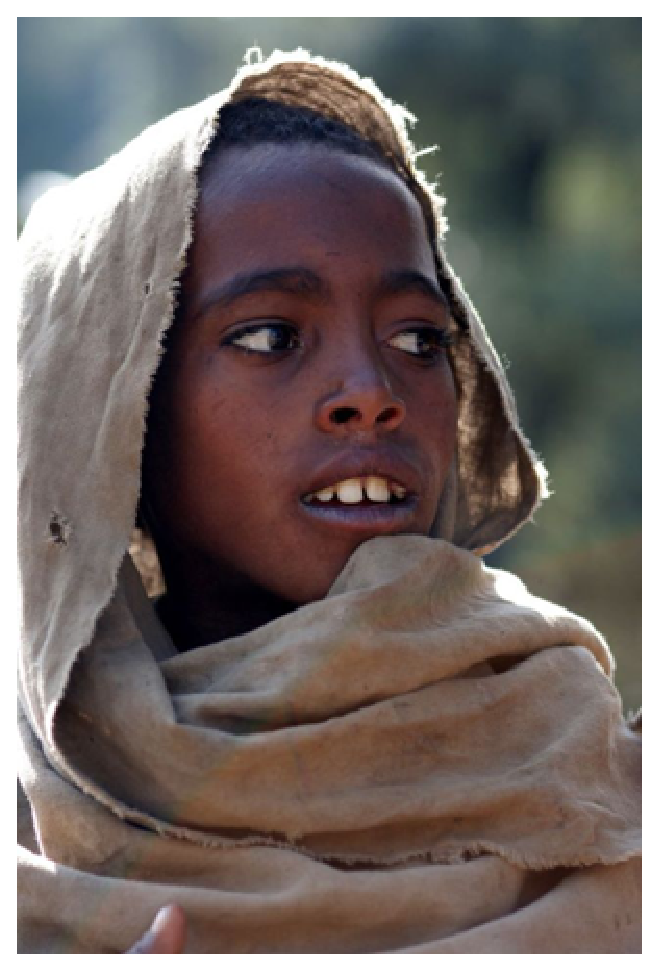
\includegraphics{etiopan.eps}
            \reflectbox{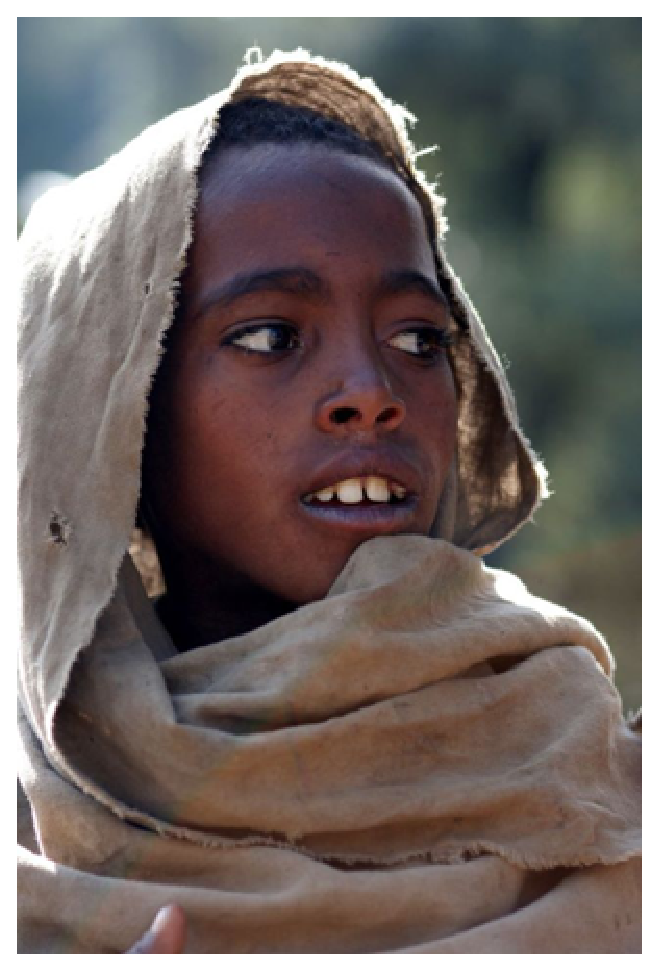
\includegraphics{etiopan.eps}}
        }
        \caption{Malý Etiopánek a~jeho bratříček}
    \label{fig:etiopan}
\end{figure}


\newpage


Rozdíl mezi vektorovým\,\dots

\begin{figure}[h]
    \scalebox{0.4}{
\includegraphics{oniisan.eps}}
    \centering
    \caption{Vektorový obrázek}
    \label{fig:vektor}
\end{figure}

\bigskip
 
\noindent \dots\,a~bitmapovým obrázkem

\begin{figure}[h]
    \scalebox{0.6}{
\includegraphics{oniisan2.eps}}
    \centering
    \caption{Bitmapový obrázek}
    \label{fig:rastr}
\end{figure}

\bigskip

\noindent se projeví například při zvětšení.

Odkazy (nejen ty) na obrázky 1, 2 a 3, na tabulky 1 a 2 a také na algoritmus 1 jsou udělány pomocí křížových odkazů. Pak je ovšem potřeba zdrojový soubor přeložit dvakrát.
Vektorové obrázky lze vytvořit i přímo v \LaTeX u, například pomocí prostředí \verb|picture|.

% kresleni domu - na sirku
\begin{landscape}
        \begin{figure}[h]
            \setlength{\unitlength}{1mm}
            \centering
            \begin{picture}(200, 110)
                % obrys
                \linethickness{1pt}
                \put(0, 0){\framebox(200, 100){}}

                % znarorneni zeme
                \linethickness{1.5mm}
                \put(4,14){\line(1,0){192}}

                % domecek
                \linethickness{0.4mm}
                \put(24, 74){\line(1, 0){36}}
                \put(60, 14){\line(0, 0){60}}
                \put(60, 50){\line(1, 0){60}}
				\put(24, 14){\line(0, 0){60}}
				\put(120, 14){\line(0, 0){36}}

                %garaz
                \put(28, 50){\line(1, 0){28}}
                \put(28, 14){\line(0, 0){36}}
                \put(56, 14){\line(0, 0){36}}

                %dvere
                \put(70, 14){\line(0, 0){22}}
                \put(79, 14){\line(0, 0){22}}
                \put(70, 36){\line(1, 0){9}}

                %okno2
                \put(90, 22){\line(0, 0){22}}
                \put(110, 22){\line(0, 0){22}}
                \put(90, 44){\line(1, 0){20}}
                \put(90, 22){\line(1, 0){20}}
    
                % slunce
                \put(140, 80){\circle{14}}
        \end{picture}
        \caption{Vektorový obrázek moderního bydlení vhodného pro 21. století. (Buď to vytvořte stejný obrázek, anebo nakreslete pomocí picture váš vlastní domov.)}
        \label{landscape:house}
    \end{figure}
\end{landscape}

\end{document}
